\chapter{Resultados}

Neste capitulo pretende-se..... 


\section{Testes na API REST}

De modo a testar a API REST foram utilizadas duas ferramentas, sendo a primeira gráfica e a segunda para linhas de comandos: 

\begin{itemize}
	\item \textit{Advanced REST client} \footnote{\url{https://advancedrestclient.com/}}: consiste numa ferramenta gráfica que permite 
	\item CURL: 
\end{itemize}





\begin{figure}[h]
	\centering
	\begin{minipage}[b]{0.49\textwidth}
		\centering
		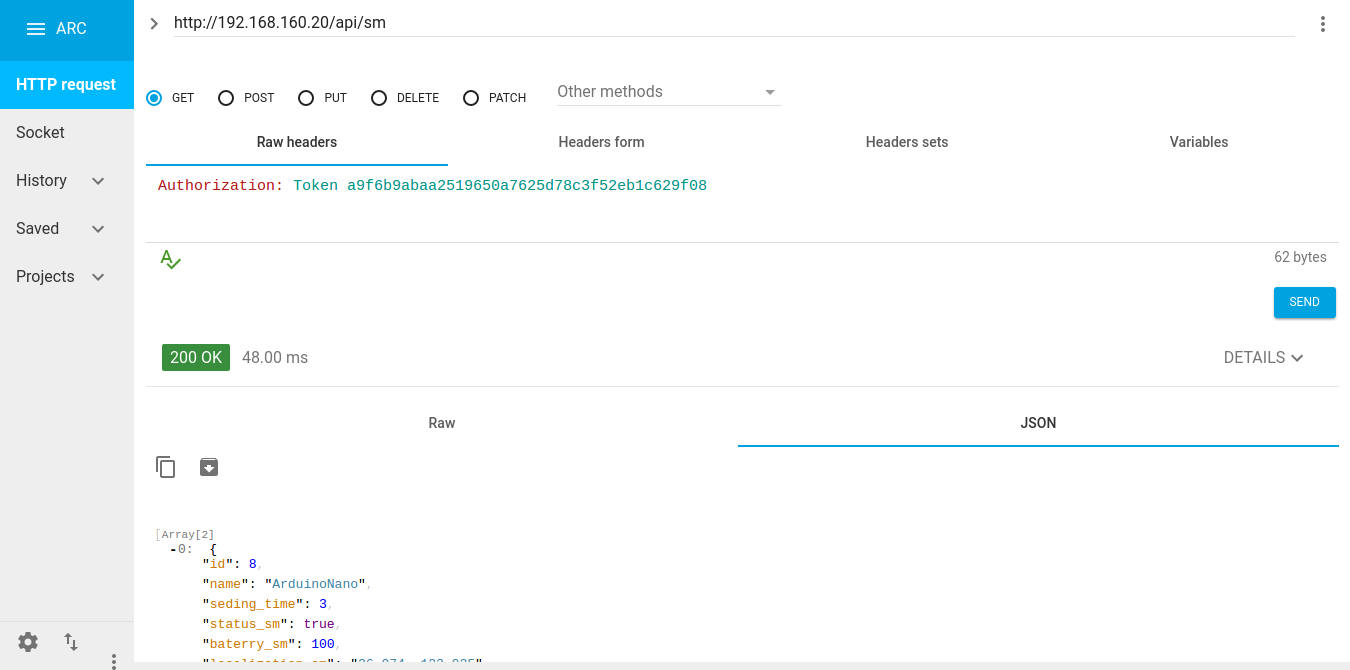
\includegraphics[width=\textwidth]{prints-web/API_teste1.png}
		\caption{Sensor TTC 104 NTC}
	\end{minipage}
	\hfill
	\begin{minipage}[b]{0.49\textwidth}
		\centering
		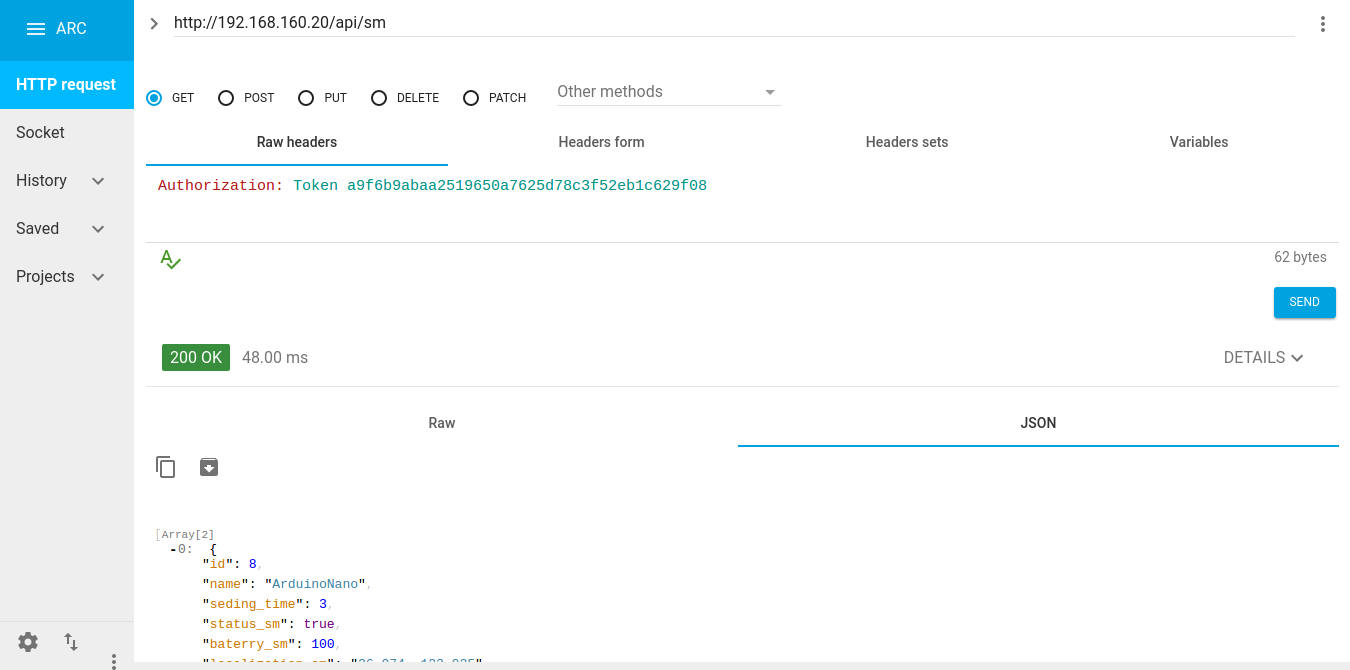
\includegraphics[width=\textwidth]{prints-web/API_teste1.png}
		\caption{Retirado de \cite{Rosebrock2015}}
		\label{esquema-temp}
	\end{minipage}
\end{figure}



O programa auxiliar de desenvolvedores da web para criar e testar solicitações HTTP personalizadas.
Uma melhor ferramenta de teste da API!

Economize seu tempo com a ferramenta de teste API mais fácil por aí. Sem formulários e scripts complicados. Fácil de usar, mas muito poderoso.

O único cliente REST que faz a conexão diretamente no soquete, dando-lhe controle total sobre os cabeçalhos de conexão e solicitação / resposta.

Nota: Você deve usar o certificado válido (para conexões seguras) para usar este aplicativo. Obtenha certificado SSL gratuito do http://www.crypt.org. Alternativamente, verifique "usar XHR" para desativar o soquete e usar a conexão regular do Chrome.
Você pode configurar o proxy nas configurações do Chrome se tiver problemas para conectar a máquina remota.

Para executar o aplicativo, vá para Nova guia, clique em "Aplicativos" na barra superior e encontre o ícone ARC. O aplicativo também se instala na pesquisa de aplicativos do sistema. No MacOS é comando + espaço, no Windows é um botão do Windows. Digite o nome do aplicativo para encontrar o aplicativo.

O que há de novo:
- Atualização de banco de dados. Agora, a história e os salvos serão muito mais rápidos
- Request history explorer - quando você lembram um histórico / pedido salvo, você verá um histórico dos pedidos que mede para este ponto final
- Novos conjuntos de cabeçalho - defina conjuntos de cabeçalho próprios e use-os com seus pedidos
%- Editor de variáveis ​​e variáveis ​​- você pode definir suas próprias variáveis ​​e colocá-las no painel de solicitação

Características:
- Integrado com o Google Drive
- Solicitações feitas em soquetes, o que lhe dá mais controle sobre cabeçalhos HTTP
- Cabeçalhos HTTP e editor de carga útil
- WebSockets!
- ajuda no preenchimento de cabeçalhos HTTP (sugestão + conclusão do código)
- adicionar lista de cabeçalhos como dados brutos ou via formulário
- construa o corpo POST ou PUT através de entrada, formulário ou arquivo de envio bruto com solicitação
- definir codificação de formulário personalizado
- lembre-se da última solicitação (salve o estado atual do formulário e restaure na carga)
- salvar (Ctrl + S) e abrir (Ctrl + O) formulários de solicitação salvos
- história dos pedidos
- importação / exportação de dados

Informe problemas em https://github.com/jarrodek/ChromeRestClient/issues
Política de privacidade: https://docs.google.com/document/d/1BzrKQ0NxFXuDIe2zMA-0SZBNU0P46MHr4GftZmoLUQU/edit?usp=sharing



\section{Interface web}


A Web-based User Interface was created, which fully demonstrates the MDM capabilities
and system management. The interface displays at all moments the alias and address of the
current logged user.
Through the UI it is possible to:

\section{Interface mobile}





\section{Simulação em hardware}


\section{Sistema de deteção de intrusos}

